\chapter{Evaluation}\label{chapter:evaluation}

In this chapter we evaluate our student model on a number of downstream tasks.
We train a student model with the best performing hyperparameters' values from
Chapter~\ref{chapter:experiments} on a large text corpora. We then evaluate this
final model on a set of 8 document downstream tasks. We simulate a scenario
where there are no data to train a dedicated model on or finetune a pre-trained
embedding model. In our opinion this is where a generic pre-trained embedding
model is most valued and we therefore focus on evaluating embedding models for
this exact use case. We also use the same checkpoint for all types of tasks to
highlight the usability of our model in different use cases.

\section{Our model}

TODO: think of a name, so we are not constantly labelling it "our"
% - set of major hyperparameters (all hyperparameters in an appendix)

% Incorporate section from experiments about training the final PV
% \subsubsection{Training the contextual teacher}

% We take the best performing hyperparameter values from the previous section and
% train the model on a large corpora. As we later train our student model with the
% contextual teacher's outputs, each piece of data we train our contextual model
% with, is effectively also part of the student's training data. Therefore we
% construct the PV training dataset similarly as \Dataset{val\_500k}: we evenly
% sample English Wikipedia articles and RealNews \citep{zellers2019defending}
% articles with more than 1200 Longformer tokens. We do so for the same reasons
% that were mentioned in Section~\ref{section:val_training_data}.

% Since PV is a small model and is able to process data very quickly during
% training, we can afford to use all of the RealNews articles that are long enough
% and an equal amount of Wikipedia articles. This results in a corpus that has
% 8.3M documents. We train the model for 10 epochs, but restrict the maximum
%   vocabulary size to $1.2{\times}10^7$ words to limit the memory footprint to
%   roughly 140~GB.

\subsection{Training data}

% - training data
%   - why we use such data
%   - statistics (lengths)

% Explanation why we use the same data
% We do so, to highlight the benefits of our method when we compare the two
% models. If we used different data instead, the two models would not be as easily
% comparable since any gain or loss of performance could be attributed either to
% the training data or to our method.

We train our student model on a corpus of long documents. We train our student
model on the same data that were used to train Longformer. By using the data our
student model was already trained on, we eliminate the possibility that the
training data were the key ingredient and the cause of the performance gain or
loss of our student model. Instead, our training method is to be blamed or given
credit. Following Longformer's approach, we use the English
Wikipedia\footnote{\url{https://huggingface.co/datasets/wikipedia/viewer/20220301.en}}
and documents from Realnews dataset~\citep{zellers2019defending} that have above
1200 Longformer's tokens. We mix both sources equally, by randomly sampling from
     both datasets. Because Wikipedia does not have a validation split, we
     sample the validation documents again from its train split, avoiding
     already chosen training documents. We label the resulting dataset as
     \Dataset{train\_1500k} to clearly identify it. As can be seen in the
     Table~\ref{table:train_data_stats}, \Dataset{train\_1500k} contains 1.5
     million long documents out of which only about 30\% can be processed by our
     structural teacher whole. Though \Dataset{train\_1500k}'s length
     distribution, which is depicted in Figure~\ref{fig:train_data_ecdf}, is far
     from uniform.

\begin{table}
    \centering
\begin{tabular}{lrr}
\toprule
Split & Train & Validation \\
\midrule
Documents & 1 500 000 & 30 000 \\
Tokens & 2.06e+09 & 4.15e+07 \\
Avg. tokens per document & 1374.18$\pm$1736.64 & 1382.12$\pm$1697.09 \\
SBERT tokens over 384 & 70.54\% & 70.73\% \\
SBERT tokens over 512 & 66.36\% & 66.84\% \\
\bottomrule
\end{tabular}

    \caption{Statistics of \Dataset{train\_1500k}. For each split we also show
    the percentage of documents with the number of SBERT tokens above given
    threshold.}

    \label{table:train_data_stats}

\end{table}

\begin{figure}
    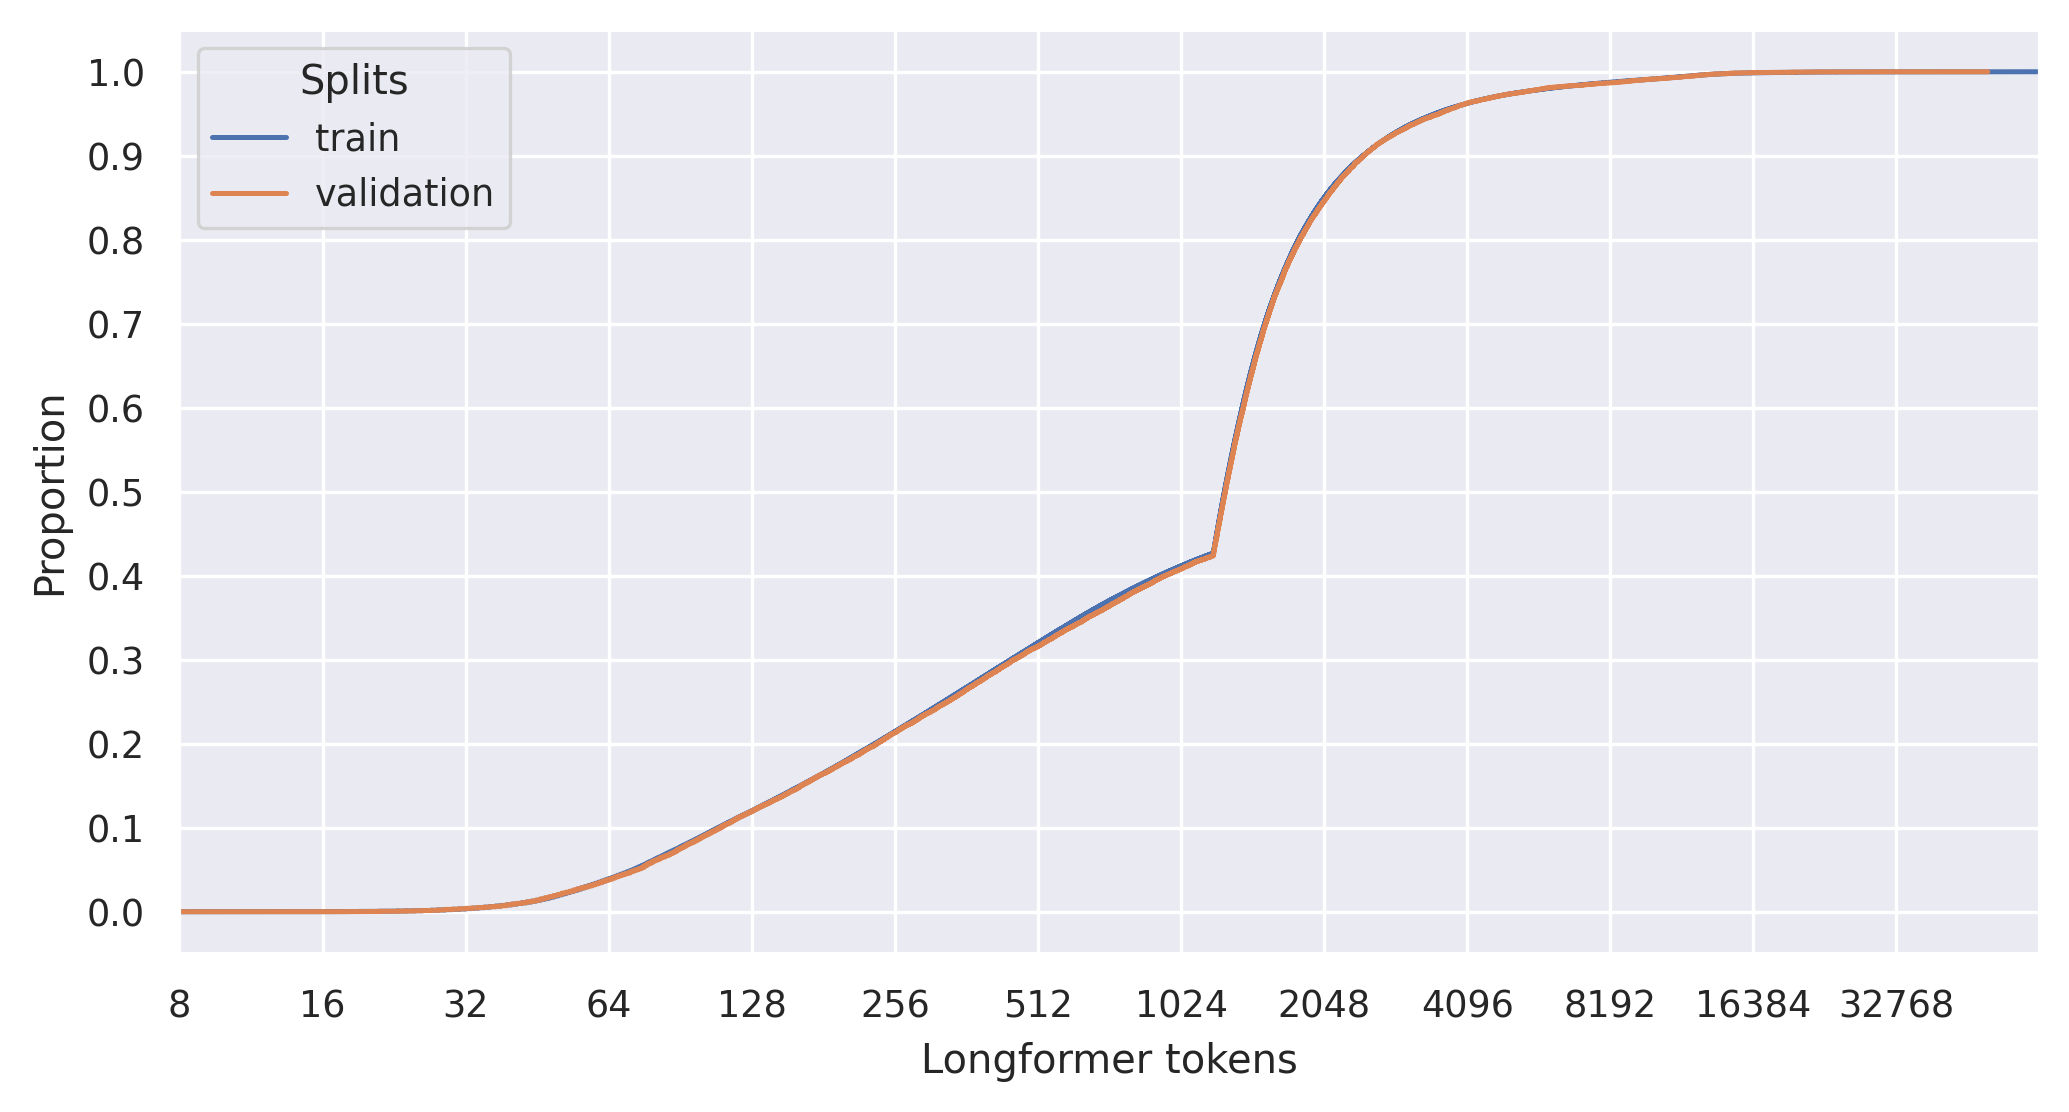
\includegraphics[width=\textwidth]{./img/train_data_ecdf.png}

    \caption{Estimated cumulative distribution function of number of Longformer
    tokens per document in \Dataset{train\_1500k}.}

    \label{fig:train_data_ecdf}
\end{figure}


% \section{Results}

% split to classification and similarity-based
% - for each subsection
%   - introduce the tasks
%   - say how we evaluate -- metric, finetuning params
%   - give results in a table format
% - for each task
%   - say why we picked it
%   - what is it


% - how we pick the tasks
% - list of the tasks with brief description
%   - associated metric
%   - how do we evaluate it
% - table with all the dataset statistics

% We evaluate our embedding model on a set of 6 classification and 2
% similarity-based downstream tasks. When picking tasks we paid special attention
% to the length of documents. Our goal was to cover a range of input's lengths
% to demonstrate the effects of our training for given length....?

% TODO: come back to this once the results are in, it might happen the lengths
% don't correspond to performance (like in validation) so this talk may be
% worthless


\section{Classification tasks}

Classification is a typical type of evaluation task for a textual embedding. In
our evaluation set we cover several use cases including classification based on
sentiment, on content, as well as citation and plagiarism detection. Our
evaluation set also contains large span of document lengths from the very short
texts having just over 100 tokens to extremely long with about 12 thousand
tokens. An overview of our classification tasks is displayed in
Table~\ref{table:evaluation_tasks_overview} and their splits' statistics in
Table~\ref{table:evaluation_tasks_stats}. We also plot the length distribution
of all tasks in Figure~\ref{fig:eval_task_longformer_token_dist} to show how
well the tasks cover the range of document lengths.

We use a heavily regularized neural network as a classifier for each task. The
classifier gets an embedding or a concatenation of two embeddings, in case of
document pair classification, and is trained with a cross entropy loss to
classify its input. We provide all the relevant hyperparameters in
Table~\ref{table:head_train_eval_params}. For all task we use accuracy as the
evaluation metric. For tasks with more classes we use micro averaging to give
each input the same weight.

We do not finetune the embedding model for each task. While it could increase
the performance, finetuning the embedding model for each task makes it more
difficult to estimate the benefits of our training method.

% The tasks from the first group are inherently
% less difficult, because the classifier just needs to find a piece of
% information in an embedding. On the other hand, in the task from the second
% group, the classifier must compare two embeddings and

\begin{table}
    \centering
    \begin{tabular}{llrrr}
        \toprule
        \multicolumn{3}{c}{} & \multicolumn{2}{c}{Class percentage} \\
        \cline{4-5}
        Dataset & Inputs & Classes & Train & Test \\
        \midrule
        \Task{arxiv} & documents & 11 & 9.09$\pm$1.25\% & 9.09$\pm$1.30\% \\
        \Task{imdb} & documents & 2 & 50.00$\pm$0.00\% & 50.00$\pm$0.00\% \\
        \Task{oc} & pairs of documents & 2 & 50.00$\pm$0.07\% & 50.00$\pm$0.34\% \\
        \Task{aan} & pairs of documents & 2 & 50.00$\pm$1.50\% & 50.00$\pm$0.77\% \\
        \Task{s2orc} & pairs of documents & 2 & 50.00$\pm$0.09\% & 50.00$\pm$0.33\% \\
        \Task{pan} & pairs of documents & 2 & 50.00$\pm$0.00\% & 50.00$\pm$0.00\% \\
        \bottomrule
    \end{tabular}

    \caption{Overview of our classification tasks. Each task classifies either
    documents or pairs of documents into several classes. We also show the mean
    and the standard deviation of percentage of class label within a given
    split.}

    \label{table:evaluation_tasks_overview}

\end{table}

\begin{table}
    \centering
    \begin{tabular}{llrrr}
        \toprule
        Dataset & Split & Documents & Tokens over 384 & Tokens over 512 \\
        \midrule
        \multirow[c]{2}{*}{\Task{arxiv}} & Train & 28 388 & 100.00\% & 100.00\% \\
        & Test & 2 500 & 100.00\% & 100.00\% \\
        \cline{1-5}
        \multirow[c]{2}{*}{\Task{imdb}} & Train & 25 000 & 24.56\% & 14.68\% \\
        & Test & 25 000 & 23.54\% & 13.95\% \\
        \cline{1-5}
        \multirow[c]{2}{*}{\Task{oc}} & Train & 240 000 & 12.31\% & 1.07\% \\
        & Test & 30 000 & 12.24\% & 1.02\% \\
        \cline{1-5}
        \multirow[c]{2}{*}{\Task{aan}} & Train & 106 592 & 0.37\% & 0.06\% \\
        & Test & 13 324 & 0.45\% & 0.08\% \\
        \cline{1-5}
        \multirow[c]{2}{*}{\Task{s2orc}} & Train & 152 000 & 33.24\% & 18.67\% \\
        & Test & 19 000 & 32.96\% & 18.20\% \\
        \cline{1-5}
        \multirow[c]{2}{*}{\Task{pan}} & Train & 17 968 & 69.93\% & 59.45\% \\
        & Test & 2 906 & 60.82\% & 47.37\% \\
        \cline{1-5}
        \bottomrule
    \end{tabular}

    \caption{Statistics of splits of our classification evaluation tasks. For
    each task and split we include the percentage of documents with SBERT
    tokens above a given threshold. This illustrates how many documents can our
    structural teacher process as a whole and how many documents need to be
    truncated.}

    \label{table:evaluation_tasks_stats}

\end{table}

\begin{figure}
    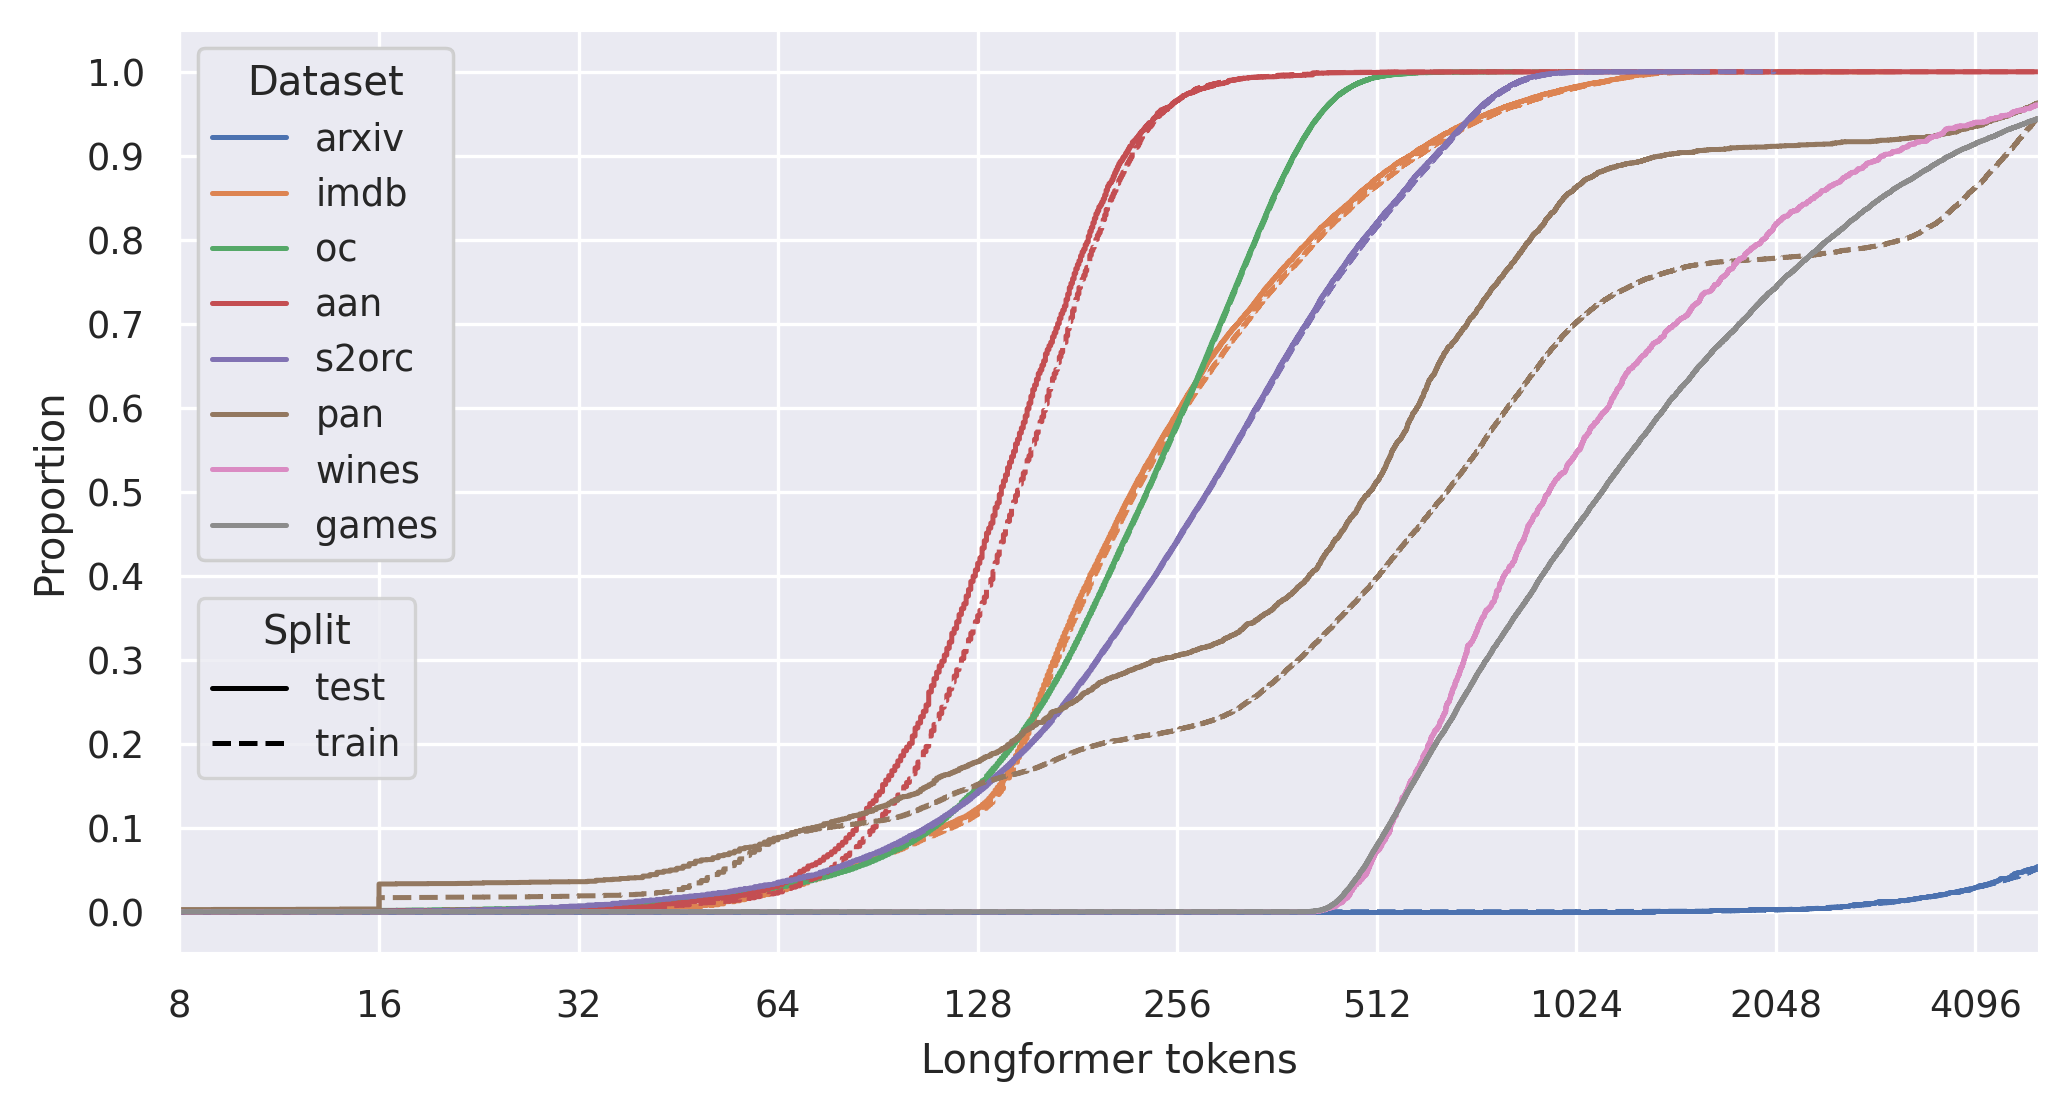
\includegraphics[width=\textwidth]{./img/eval_tasks_token_ecdf.png}

    \caption{Estimated cumulative length distribution of the number of
    Longformer tokens in a document.}

    \label{fig:eval_task_longformer_token_dist}
\end{figure}


\begin{table}
  \centering
  \begin{tabular}{l c}
    \toprule
    Parameter & Value \\
    \midrule
    Hidden features & 50 \\
    Hidden dropout rate & 0.5 \\
    Hidden activation & ReLU \\
    Epochs & 30 \\
    Batch size & 32 \\
    Weight decay & 0.1 \\
    Label smoothing & 0.1 \\
    Learning rate & 1e-4 \\
    Learning rate decay & Cosine \\
    Maximum gradient norm & 1.0 \\
    Optimizer & AdamW \\
    Mixed-precision training & Yes \\
    \bottomrule
  \end{tabular}

  \caption{Parameters for training classification heads during evaluation.}
  \label{table:head_train_eval_params}
\end{table}

\subsection{Tasks' descriptions}

\subsubsection{IMDB movie reviews}

The IMDB dataset~\citep{maas2011learning} (denoted as \Task{imdb}) is a binary
classification dataset that is quite frequently included in evaluation of
long-context NLP models~\citep{zaheer2020big, beltagy2020longformer,
le2014distributed}. The datasets consists of movie reviews, each with associated
rating on a 10 point scale. The reviews that rated the movie with 7 points or
higher are classified as positive, and reviews with less than 4 points are
classified as negative. For each movie there can be up to 30 reviews and the
test set contains disjoint set of movies. Along with the train and test splits
the dataset contains also an unsupervised split without any rating or class
labels. While the majority of the reviews are shorter; around 25\% of documents
are longer than the maximal context of our structural teacher and around 14\%
being longer than 512 tokens. Consequently, we use IMDB dataset to gain an
estimate of the performance of our model on short to medium documents.

\subsubsection{Arxiv papers}

Arxiv papers~\citep{arxiv_papers} (denoted as \Task{arxiv}) is a collection of
papers from ArXiv\footnote{\url{arxiv.org}} -- online archive of scholary
papers. Each paper contains its full text spanning at least 1000 words. The
longest papers are truncated to 10000 words. The papers are classified to 11
groups, that correspond to the scientific field of the paper. Since each paper
can be associated with several scientific fields a small portion of the
documents ($\approx$~3.1\%) appears more than once, but with different label
each time. The scientific fields cover mainly fields of Computer science such as
Artificial intelligence or Data structures but also fields connected with
Mathematics such as Group theory or Statistics theory. The classes are not quite
balanced with the most numerous class having around 12\% of documents, while the
least numerous class only having around 7\%. \Task{arxiv} represents the extreme
case of very long documents. As 97\% of the dataset's documents are longer than
the maximum context length of our student model.

\subsubsection{ACL Anthology Network Corpus citations}

The ACL Anthology Network Corpus citations dataset~\citep{zhou2020multilevel}
(denoted as \Task{aan}) is a citation prediciton dataset. Each example in the
dataset contains a pair of paper's abstracts and is classified as positive if
the first document cites the second one, or negative if it does not. The dataset
is compiled from the ACL Anothology Network Corpus~\citep{radev2013acl}, where
each source paper creates positive pairs with all cited papers and negative pair
with one other randomly sampled non-cited paper. The focus of this dataset is on
very short documents; just around 4\% of documents are longer than 256 tokens.
\Task{aan} has the shortest documents of all datasets in our evaluation set.

\subsubsection{Semantic Scholar Open Corpus citations}

The Semantic Scholar Open Corpus citations dataset~\citep{zhou2020multilevel}
(denoted as \Task{oc}) is also a citation prediction dataset in the same format
as \Task{aan}. As the dataset name suggests it was compiled from the Semantic
Scholar Open Corpus~\citep{bhagavatula2018content}. In this dataset, only a
single positive pair is generated for each source paper, which results in much
higher count of unique papers in the dataset compared to \Task{aan}. \Task{oc}
contains relatively shorter sequences with only 12\% of documents larger than
the maximum context of our structural teacher.

\subsubsection{Semantic Scholar Open Research Corpus citations}

The Semantic Scholar Open Research Corpus citations
dataset~\citep{zhou2020multilevel} (denoted as \Task{s2orc}) is our third and
final citation prediciton dataset. The source of this dataset is the Semantic
Scholar Open Research Corpus~\citep{lo2019s2orc} where each paper is divided
into sections that are connected via links to papers cited within the given
sections. This structure is used to generate positive and negative pairs in the
citation dataset \Task{s2orc}. A section is paired with an abstract of cited
paper to create a positive pair and with an abstract of non-cited paper to
create a negative pair.

The documents in \Task{s2orc} are comparatively longer than those of the
previously mentioned tasks, except for \Task{arxiv}, with over 50\% of document
being longer than 256 tokens.

\subsubsection{PAN plagiarism detection}

The final classification dataset is the PAN plagiarism detection
dataset~\citep{zhou2020multilevel} (denoted as \Task{pan}). It was constructed
from PAN plagiarism alignment task~\citep{potthast2013overview}, which is a
collection of pairs of web documents, where the sections relevant to plagiarism
are humanly annotated both in the source as well as in the suspicious document.
\Task{pan} is a binary classification task where each document pair is
classified as positive or negative. Positive inputs pair the source's
plagiarised section with a part of the suspicious document containing the
corresponding plagiarised section. Negative pairs are constructed from the
positives one by replacing the source's segment by different part of the same
document that is not annotated as being plagiarised. \Task{pan} contains longer
documents; around 60\% are longer than the maximum context size of our
structural teacher and just under 50\% of document are longer than 512 tokens.
\Task{pan} therefore creates an intermediate step between documents of medium
length in tasks such as \Task{imdb} or \Task{s2orc} and extremely long documents
in \Task{arxiv}.

\subsection{Results}

\section{Similarity-based tasks}

Besides from classification tasks we also evaluate our model on two tasks that
are based on similarity metrics between two embeddings. Our evaluation set
focuses on long Wikipedia articles from two different fields of interest. The
statistics of similarity-based tasks are displayed in
Table~\ref{table:eval_sims_tasks}. The distribution of documents' lengths is
plotted in Figure~\ref{fig:eval_task_longformer_token_dist}.

We use cosine as a measure of embeddings' closeness. Same as with the
classification tasks, here we also do not finetune the embeddings to a given
task. Consequently, we do not need training or validation splits and we can use
the whole datasets for evaluation. Our main scoring metric is Mean Average
Precision (\emph{MAP}), but we also present Mean Reciprocal Rank (\emph{MRR}).
While MAP scores the whole predicted ordering, MRR is more interpretable and can
be more important in scenarios where we care only about the first positive
result.

\begin{table}
  \centering
  \footnotesize
  \begin{tabular}{lrrrrr}
  \toprule
    Dataset & Documents & Sources & Targets per source & Tokens over 384 & Tokens over 512 \\
    \midrule
    \Task{wines} & 1 662 & 89 & 8.92$\pm$1.23 & 100.00\% & 90.43\% \\
    \Task{games} & 21 228 & 88 & 8.74$\pm$2.35 & 100.00\% & 91.78\% \\
    \bottomrule
  \end{tabular}

  \caption{Statistics of our similarity-based evaluation tasks. Each dataset is
  composed of several source documents each with a set of similar target
  documents. Additionally we show the percentage of documents with SBERT tokens
  above a given threshold to highlight how many documents need to be truncated
  in order to be processed by our structural teacher.}

  \label{table:eval_sims_tasks}

\end{table}

\subsection{Tasks' description}

\subsubsection{Wines and Video games Wikipedia articles}

Both of our similarity-based tasks are datasets consisting of Wikipedia
articles from two fields of interests: wines (denoted as \Task{wines}) and
video games (denoted as \Task{games})~\citep{ginzburg2021self}. Each dataset
contains around 90 source articles each associated with around 10 similar
articles. We find the two datasets very unique as they combine two aspects
which are rarely seen together. First the similarities are based on human
annotations and not on proxy measures such as common citations or outgoing
links. Second the documents are relatively long with around 90\% of documents
being longer than 512 tokens.

\subsection{Results}

% \section{Tasks}

% Each task aims to test a different aspect of a model. Our aim was to design a
% set of tasks, which can capture a model's capability to embed whole documents.
% The major obstacle we faced was the lack of labeled datasets with longer pieces
% of text (more than 512 tokens).

% TODO: how did we solve the issue

% TODO: complete list of task types

% \subsubsection{Classification}

% Classification tasks test model's capability to separate inputs based on a
% complex feature. In our settings, classification tasks can tell us what
% information the document embedding contains.


% \subsection{IMDB Sentiment Analysis}

% IMDB sentiment analysis task is a simple binary classification task. The dataset
% contains movie reviews from the Internet Movie
% Database\footnote{\url{www.imdb.com}} labeled as either positive or negative.
% The dataset is commonly referred to as IMDB classification or sentiment
% dataset~\cite{maas11}.

% The dataset is split evenly to test and train set, each having 25000 reviews.
% The dataset also contains 50000 unlabeled reviews. The label distribution in
% both sets is uniform, each of of the two labels is represented by 12500 reviews.

% As can be seen from the figure Figure~\ref{fig:imdb_word_token_dist} the reviews
% are quite short with only 13.56\% being longer than 512 RoBERTa tokens.

% \begin{figure}[ht]
%   \centering
%   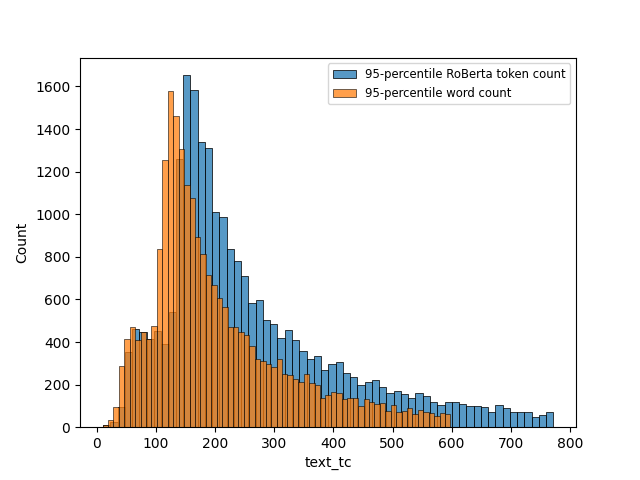
\includegraphics[width=0.9\textwidth]{img/imdb_word_token_distributions.png}
%   \caption{Word count and token count distribution of 95-percentiles of
%   reviews. The tokens are generated using RoBERTa's pretrained tokenizer from
%   HuggingFace}\label{fig:imdb_word_token_dist}
% \end{figure}

% We included this task to see how our model compares in relatively undemanding
% settings, while also evaluating its performance on shorter documents.
